\subsubsection{Security and Authentication}

Regarding the security architecture design, the implementation is streamlined through \texttt{Microsoft.Identity.Web} library, which provides seamless integration with Azure Active Directory and simplifies JWT bearer token validation. The authentication middleware is configured in the application startup file (\texttt{Program.cs}) as shown in Figure \ref{fig:program-file-auth}.

\begin{figure}[H]
    \centering
    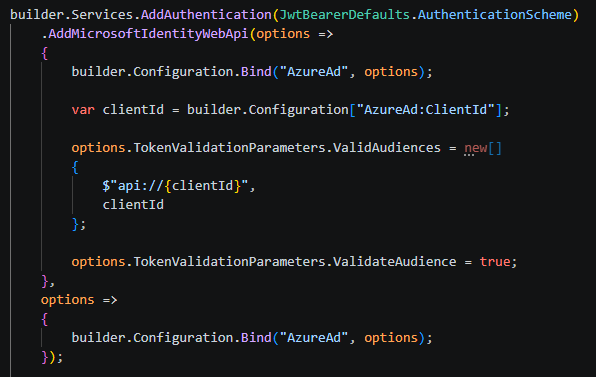
\includegraphics[width=0.7\textwidth]{Images/Implementation/ProgramFileAuth.png}
    \caption[Authentication middleware configuration in Program.cs]
    {Authentication middleware configuration in \texttt{Program.cs}. [Own creation]}
    \label{fig:program-file-auth}
\end{figure}

This configuration registers the JWT Bearer authentication scheme and integrates it with Azure AD through the \texttt{Microsoft.Identity.Web} library. The Azure AD settings are loaded from the application configuration, while the token validation parameters are customized to accept \texttt{api://{clientId}} and the Client ID as valid audiences. Audience validation ensures that only tokens intended for this API are accepted. With this configuration, the connection with the required middleware is established to automatically validate the JWT bearer token included in the \texttt{Authorization} header of incoming requests.

To protect the API endpoints, it is sufficient to simply add an \texttt{[Authorize]} (see Figure \ref{fig:authorize-controller})  attribute at the top of the controller classes. This attribute restricts resource access to exclusively authenticated users.


\begin{figure}[H]
    \centering
    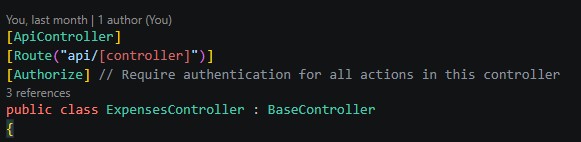
\includegraphics[width=0.7\textwidth]{Images/Implementation/AuthorizeController.png}
    \caption[Authorization attribute configuration in ExpensesController.cs]
    {Authorization attribute configuration in \texttt{ExpensesController.cs}. [Own creation]}
    \label{fig:authorize-controller}
\end{figure}



